%%%%%%%%%%%%%%%%%%%%%%%%%%%%%%%%%%%%%%%%%%%%%%%%%%%%%%%%%%%%%%%%%%%%%%
% MATH 2007 - Calculus II Review
% by Simon Pratt
%%%%%%%%%%%%%%%%%%%%%%%%%%%%%%%%%%%%%%%%%%%%%%%%%%%%%%%%%%%%%%%%%%%%%%
\documentclass{article}

\usepackage{fullpage}
\usepackage{parskip}
\usepackage{amsmath}
\usepackage{titlesec}
\usepackage{graphics}

\newcommand{\sectionbreak}{\clearpage}

\title{MATH 2007 Review}
\author{Simon Pratt}
\date{\today}



%%%%%%%%%%%%%%%%%%%%%%%%%%%%%%%%%%%%%%%%%%%%%%%%%%%%%%%%%%%%%%%%%%%%%%
% New Square Root
%%%%%%%%%%%%%%%%%%%%%%%%%%%%%%%%%%%%%%%%%%%%%%%%%%%%%%%%%%%%%%%%%%%%%%
% it renames \sqrt as \oldsqrt
\let\oldsqrt\sqrt
% it defines the new \sqrt in terms of the old one
\def\sqrt{\mathpalette\DHLhksqrt}
\def\DHLhksqrt#1#2{%
\setbox0=\hbox{$#1\oldsqrt{#2\,}$}\dimen0=\ht0
\advance\dimen0-0.2\ht0
\setbox2=\hbox{\vrule height\ht0 depth -\dimen0}%
{\box0\lower0.4pt\box2}}

\begin{document}

{\Huge MATH 2007 Review}

\vspace{1 cm}

{\huge Topics Covered}

{\tiny Section numbers are from Nelson's custom text book for the course}

Test 1
\begin{itemize}
\item 4.5 Integration by Substitution
\item 8.2 Integration by Parts
\item 8.3 Trigonometric Integrals
\item 8.4 Trigonometric Substitution
\end{itemize}

Test 2
\begin{itemize}
\item 8.5 Partial Fractions
\item 8.7 Indeterminate Forms and L'H\^{o}spital's Rule
\item 8.8 Improper Integrals*
\item 10.2 Plane Curves and Parametric Equations
\end{itemize}

Test 3
\begin{itemize}
\item 10.3 Parametric Equations and Calculus
\item 10.4 Polar Coordinates and Polar Graphs
\item 10.5 Area and Arc Length in Polar Coordinates*
\item 9.1 Sequences
\end{itemize}

Test 4
\begin{itemize}
\item 9.2 Series and Convergence
\item 9.3 The Integral Test and p-Series
\item 9.4 Comparisons of Series*
\item 9.5 Alternating Series
\end{itemize}

Final Exam
\begin{itemize}
\item 9.6 The Ratio and Root Tests*
\item 9.7 Taylor Polynomials and Approximations*
\item 9.8 Power Series
\item 9.9 Representation of Functions by Power Series*
\item 9.10 Taylor and Maclaurin Series
\end{itemize}

{\tiny *could not remember offhand}

\section{Integration by Substitution}

When we are presented with an integral that is the product of a
function with its derivative, we can substitute the function for a new
variable and its derivative for the differential of that variable.

For example:

\[
\int \frac{dx}{xlnx}
\]

We know the derivative of $lnx$ is $\frac{1}{x}$.  Let $u=lnx$,
$du=\frac{1}{x}$, then we have:

\[
\int u^{-1}du
\]

Then we can differentiate with respect to $u$ and get:

\[
ln \left| u \right| \\
\]

And substituting $u$ back in, we get:

\[
\int \frac{dx}{xlnx} = \ln \left| lnx \right|
\]

This method of integration is analagous to the chain rule for
differentiation.

\section{Integration by Parts}

Sometimes we are presented with the integral of a product of
functions, one of which gets simpler when derived and the other gets
simpler when integrated.  In this case, we can use the formula:

\[
\int udv = uv - \int vdu
\]

For example:

\[
\int xe^xdx
\]

Let $u = x$, $dv = e^x$, and thusly $du = dx$, $v = e^x$, we get:

\begin{align*}
  &xe^x - \int e^xdx \\
  = &xe^x - e^x \\
  = &e^x(x-1)
\end{align*}

This method of integration is analagous to the product rule for
differentiation.

\section{Trigonometric Integrals}

\subsection{Evaluating $\int (sinx)^m (cosx)^ndx$}

Using the identity $(sinx)^2 + (cosx)^2 = 1$ and integration by
substitution, we can solve integrals of the form $\int (sinx)^m
(cosx)^ndx$ as long as either $m$ or $n$ are odd.

For example:

\[
\int (cosx)^2(sinx)^3dx
\]

We can substitute $(sinx)^2 = 1 - (cosx)^2$ to get:

\[
\int (cosx)^2 (1-(cosx)^2) sinx dx
\]

This expands to:

\[
\int (cosx)^2 sinx dx - \int (cosx)^4 sinx dx
\]

At which point we can substitute $u = cosx$, $du = -sinx dx$:

\begin{align*}
  &\int u^2 du - \int u^4 du \\
  = &\frac{u^3}{3} - \frac{u^5}{5}
\end{align*}

And substituting $u$ back in:

\[
\frac{(cosx)^3}{3} - \frac{(cosx)^5}{5}
\]

This works similarly if the power of $cosx$ is odd.

\newpage

However, if both powers are even, we must use the half angle formulae:

\begin{align*}
  2 sinA cosB &= sin(A - B) + sin(A + B) \\
  2 sinA sinB &= cos(A - B) - cos(A + B) \\
  2 cosA cosB &= cos(A - B) + cos(A + B)
\end{align*}

Let $A=B$:

\begin{align*}
  2 sinA cosA &= 0 + sin(2A) \\
  2 (sinA)^2 &= 1 - cos(2A) \\
  2 (cosA)^2 &= 1 + cos(2A)
\end{align*}

So for example:

\begin{align*}
  &\int (sinx)^2 (cosx)^4 dx \\
  = &\int 1/2(1 - cos2x) (1 + cos2x) dx \\
  = &1/2 \int (1 + cos2x) dx - 1/2 \int cos2x (1 + cos2x) dx \\
  = &1/2 ( \int dx + \int cos2x dx - \int cos2x dx + \int (cos2x)^2 dx ) \\
  = &1/2 ( x + \int (cos2x)^2 dx ) \\
  = &1/2 ( x + \int 1/2 (1 + cos4x) dx ) \\
  = &1/2 ( x + 1/2 ( \int dx + \int cos4x dx ) ) \\
  = &1/2 ( x + 1/2 ( x + sin4x ) ) \\
  = & \frac{ 3x + sin4x }{4}
\end{align*}

\newpage

\subsection{Evaluating $\int (tanx)^m (secx)^ndx$}

Same idea using the identity:

\begin{align*}
  (cosx)^2 + (sinx)^2 &= 1 \\
  1 + (tanx)^2 &= \frac{1}{(cosx)^2} \\
  1 + (tanx)^2 &= (secx)^2
\end{align*}

Remembering:

\begin{align*}
  &\frac{d}{dx} (secx) = secx tanx \\
  &\frac{d}{dx} (tanx) = (secx)^2 \\
  &\int tanx dx = ln \left| secx \right| + C \\
  &\int secx dx = ln \left| secx + tanx \right| + C \\
\end{align*}  

For example:

\begin{align*}
  &\int (secx)^3 dx \\
  = &\int secx ((tanx)^2 + 1) dx \\
  = &\int secx (tanx)^2 dx + \int secx dx \\
\end{align*}

Then substitute $(tanx)^2 = (secx)^2 - 1$:

\begin{align*}
  &\int secx (tanx)^2 dx + \int secx dx \\
  = &\int secx ((secx)^2 -1) dx + \int secx dx \\
  = &\int (secx)^3 dx - \int secx dx + \int secx dx \\
  = &\int (secx)^3 dx
\end{align*}

\newpage

Well crap.  Okay, try again with integration by parts using $u =
secx$, $dv = (secx)^2$ and thusly $du = secx tanx$, $v = tanx$:

\begin{align*}
  &\int (secx)^3 dx \\
  = &\int secx (secx)^2 \\
  = &(secx)(tanx) - \int tanx (secx tanx) dx
\end{align*}

And we've shown about that $\int secx (tanx)^2 dx = \int (secx)^3 dx -
\int secx dx$.  So we get:

\begin{align*}
  \int (secx)^3 dx &= (secx)(tanx) - \int (secx)^3 dx + \int secx dx \\
  \int (secx)^3 dx + \int (secx)^3 dx &=
  (secx)(tanx) + ln \left| secx + tanx \right| + C \\
  2 \int (secx)^3 dx &= (secx)(tanx) + ln \left| secx + tanx \right| + C \\
  \int (secx)^3 dx &= \frac{(secx)(tanx) + ln \left| secx + tanx \right| + C}{2}
\end{align*}

\section{Trigonometric Substitution}

When we have an integral containing a square root of the sum of two
squares, we can substitute trig identities to make the integral simpler.

For example:

\section{Partial Fractions}

When we are confronted with a product of two functions in the
denominator of a fraction, we can use partial fractions to simplify.

For example:

\section{Indeterminate Forms and L'H\^{o}spital's Rule}

Common indeterminate forms are $\frac{0}{0}$, $\frac{\infty}{\infty}$
and $\infty^\infty$.

For example:

\section{Improper Integrals}

An improper integral is a definite integral either with an infinite
interval or has a discontinuity in its interval.

In the case of an integral with an infinite interval:

\[
\int^\infty_a f(x)dx = \lim_{t \to \infty} \int^t_a f(x)dx
\]

or

\[
\int^b_\infty f(x)dx = \lim_{t \to \infty} \int^b_t f(x)dx
\]

provided that these limits exist.  We can also:

\[
\int^\infty_{-\infty} f(x)dx = \int^a_{-\infty}f(x)dx + \int^\infty_a f(x)dx
\]

provided that both of the integrals are convergent.

For example

\begin{align*}
  &\int^0_{-\infty} x e^x dx \\
  = &\lim_{t \to -\infty} \int^0_t x e^x dx \\
\end{align*}

Let $u = x$, $dv = e^x$, $du = dx$, $v = e^x$:

\begin{align*}
  = &\lim_{t \to -\infty} (x e^x - \int^0_t e^x dx) \\
  = &\lim_{t \to -\infty} (xe^x]^0_t - \left[ e^x \right]^0_t) \\
  = &\lim_{t \to -\infty} ((0 - te^t) - (e^0 - e^t)) \\
  = &\lim_{t \to -\infty} (-te^t - 1 + e^t) \\
\end{align*}

\newpage

We see that $e^t \to 0$ as $t \to -\infty$, so we have:

\begin{displaymath}
  -1 + \lim_{t \to -\infty} -te^t 
\end{displaymath}

we know this is an indeterminate form ($\infty \bullet 0$), we
can use L'H\^{o}spital's Rule and get:

\begin{align*}
  &\lim_{t \to -\infty} -te^t \\
  = &\lim_{t \to -\infty} \frac{-t}{e^{-t}} \\
  = &\lim_{t \to -\infty} \frac{-1}{-e^{-t}} \\
  = &\lim_{t \to -\infty} e^{-t} \\
  = &0
\end{align*}

So:

\begin{displaymath}
  \int^0_{-\infty} x e^x dx = -1
\end{displaymath}

\section{Plane Curves and Parametric Equations}

A plane curve is when we rotate a given curve about an axis.

Parametric equations are when $x$ and $y$ are given in terms of a parameter $t$.

For example:

\section{Parametric Equations and Calculus}

If we are given $x$ in terms of $t$ then:

\begin{align*}
  x &= f(t) \\
  dx &= f'(t)dt \\
  \frac{dx}{dt} &= f'(t)
\end{align*}

and $y$ in terms of $t$:

\begin{align*}
  y &= g(t) \\
  dy &= g'(t)dt \\
  \frac{dy}{dt} &= g'(t)
\end{align*}

Then we can determine $\frac{dy}{dx}$ by:

\begin{align*}
  \frac{dy}{dx} &= \frac{ \frac{dy}{dt} }{ \frac{dx}{dt} } \\
  &= \frac{g'(t)}{f'(t)}
\end{align*}

For example:

\section{Polar Coordinates and Polar Graphs}

Polar coordinates are given as a tuple of radius and angle.  Note that
since angles are modulo 0 and the angle of a full circle ($360^o$ or
$2\pi$), coordinates for a point aren't unique.

For example:

\[
(2,\pi) = (2,3\pi) = (2,-\pi)
\]

A polar graph is radius $r$ as a function of angle $\theta$.

For example:

\[
r = a \pm b cos \theta
\]

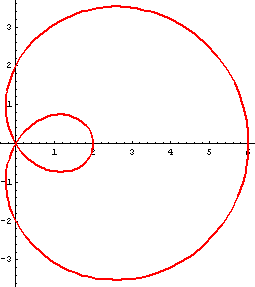
\includegraphics{Limacon}

\newpage

\[
r = cos(4 \theta)
\]

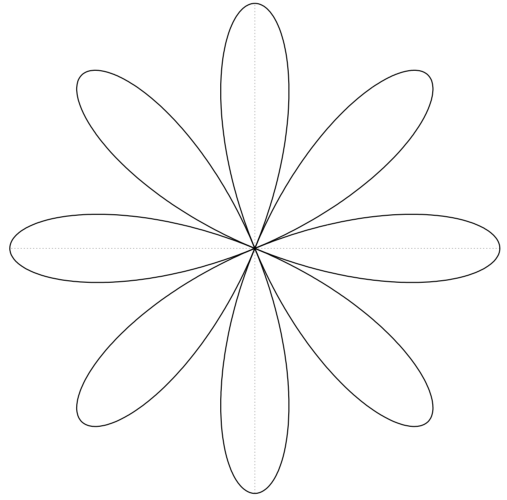
\includegraphics{Rose}

\[
r = 1
\]

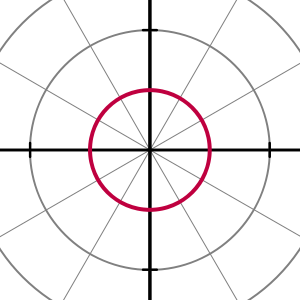
\includegraphics{Circle}

\section{Area and Arc Length in Polar Coordinates}

Formula for area: $A = \displaystyle\int^b_a \frac{1}{2} r^2 d \theta$

Formula for arc length: $L = \displaystyle\int^b_a \sqrt{r^2 + \left( \frac{dr}{d \theta} \right)^2} d \theta$

For example:

\section{Sequences}

A sequence is an ordered set of numbers, such as $1,2,3$.  A sequence
can be infinitely long such as $1,2,3,...$, and can be defined as $a_n
= n$ where $a_n$ is the $n$th term in the sequence.

For example:

\section{Series and Convergence}

A series is a sum of the numbers in a sequence, such as $1+2+3$.  A
sequence can be infinitely long, such as $1+2+3$, and can be defined
using sigma notation: $S = \displaystyle\sum_{n=1}^{\infty} f(n)$ where $S$ is the
value of the sum from 1 to infinity of the function $f(n)$.

When a the limit of the value of a series or integral as n approaches
infinity is defined and is equal to $L$, we say that the series or
integral converges to $L$.

For example:

\section{The Integral Test and p-Series}

The integral test states that given a series of the form
$\displaystyle\sum^\infty_{k=1}f(n)$, then if the integral $\displaystyle\int f(n)dn$ converges,
then the series must also converge.

A p-series is an infinite series of the form $\displaystyle\sum \frac{1}{n^p}$.
Such a series converges when $p > 1$ and diverges otherwise.

For example:

\section{Comparisons of Series}

If $a_n$, $b_n$ are both series with positive terms and $a_n$ is
bounded above by $b_n$, that is $a_n \leq b_n$ for all $n$, then if
$b_n$ converges, then $a_n$ must also converge or if $a_n$ diverges
then $b_n$ must also diverge.

For example:

\subsection{Limit Comparison Test}

If $a_n$, $b_n$ are both series with positive terms, then if

\[
\lim_{n \to \infty} \frac{a_n}{b_n} = c
\]

and $c > 0$, then $a_n$ and $b_n$ either both converge or both diverge.

For example:

\section{Alternating Series}

An alternating series is of the form $\sum (-1)^{n-1}a_n$.  A series
$\sum f(n)$ is said to be absolutely convergent if $\sum \left|
  f(n) \right|$ is convergent.  Any series which is absolutely
convergent is also convergent.

For example:

\section{The Ratio and Root Tests}

\subsection{The Ratio Test}

The ratio test shows that given $\sum a_n$, and:

\begin{align*}
  &\lim_{n \to \infty} a_n = 0 \\
  &L = \lim_{n \to \infty} \left| \frac{a_{n+1}}{a_n} \right|
\end{align*}

If $L<1$ then the series converges, if $L>1$ then the series diverges,
and if $L=1$ then the ratio test is inconclusive.

For example:

\subsection{The Root Test}

The root test shows that given $\sum a_n$, and:

\[
L = \lim_{n \to \infty} \oldsqrt[n]{\left| a_n \right|}
\]

Then if $L < 1$: $\sum a_n$ converges, if $L > 1$: $\sum a_n$
diverges and if $L = 1$: the root test is inconclusive.

For example:

\section{Taylor Polynomials and Approximations}

The formula for the $n$th Taylor polynomial at $c$ is:

$P_n(x) = \frac{f^{(n)}(c)}{n!}$

For example:

\section{Power Series}

A power series is of the form $\sum c_n(x-a)^n$.  Also, we define
$(x-a)^0$ as 1 even when $x=a$ for convenience.

Such a series is either always convergent, converges only when $x=a$
or has some radius of convergence about $x=a$.

For example:

\section{Representation of Functions by Power Series}

A function of the form $\frac{1}{1-f(x)}$ can be approximated using
the geometric series formula:

\[
\sum_{n=0}^\infty (f(x))^n = \frac{1}{1-f(x)}
\]

And the radius of convergence for this power series is $\left| f(x) \right| < 1$.

For example:

\subsection{Differentiation and Integration of Power Series}

If a power series has a radius of convergence $R > 0$, then it is
differentiable and integratable on the interval $(a-R,a+R)$.

For example:

\section{Taylor and Maclaurin Series}

A Taylor series is when function $f(x)$ can be approximated at point
$a$ with the function $\sum \frac{f^{(n)}(a)x^n}{n!}$.

For example:

\subsection{Maclaurin Series}

A special case of a Taylor series is when $a=0$, which we call a Maclaurin series.

For example:

\section{Copyright}

All following images are in the public domain or collective commons.

Limacon: https://secure.wikimedia.org/wikipedia/commons/wiki/File:Limacon.png

Rose: https://secure.wikimedia.org/wikipedia/commons/wiki/File:Rose08.png

All following images are distributed under the terms of the GNU Free Documentation License:

Circle: https://en.wikipedia.org/wiki/File:Circle\_r\%3D1.svg

\end{document}